\chapter{Theoretischer Rahmen}
Im folgenden werden die theoretischen Grundlagen erörtert, auf welchen die Anwendung basiert. In Kapitel \ref{spaced_rep} werden die Prinzipien und wissenschaftlichen Hintergründe von \textit{Spaced Repetition} thematisiert. Die Programmiersprache \textit{Dart} und das darauf basierende Framework \textit{Flutter}, mit welchem die Applikation programmiert wurde, werden in dem zweiten Kapitel \ref{dart_flutter} grundlegend nahe gebracht.

\section{Spaced Repetition}
\label{spaced_rep}
Gemerkte Informationen können laut \cite{SA:Forget} in zwei Kategorien eingeteilt werden. Entweder gehören sie zur \textit{familarity}- oder zur \textit{recollection}-Darstellung. Bei ersterem kann sich an die Information erinnert werden, diese aber nicht in Kontext mit den dazugehörigen Informationen gebracht werden. Ein bekanntes Beispiel dazu wäre, dass einem bekannten Gesicht kein Namen zuordnen werden kann. Die andere Möglichkeit ist die \textit{recollection}-Darstellung, bei welcher sich auch an den jeweiligen Kontext erinnert werden kann. Angewendet auf das vorherige Beispiel, kann sich in diesen Fall an den Namen und weitere personenbezogene Informationen erinnert werden \cite{SA:Forget}.

Beide Darstellungen von Informationen werden im Gehirn durch Neuronen gespeichert. Durch Assoziationen werden die Neuronen mithilfe von synaptischen Verbindungen angeregt. Die Assoziationen sind bei jeder Erinnerung unterschiedlich und können von Farben und Tönen bis zu mathematischen Formeln gehen. Eine synaptische Verbindung ist nicht statisch und kann im Laufe der Zeit stärker und schwächer werden. Ein zusätzlicher Faktor ist, dass Neuronen, die andere Neuronen aktivieren, mit der Zeit effektiver darin werden, andere Neuronen zu aktivieren. Das bedeutet, dass Assoziationen schneller zugehörige Reaktionen auslösen und Kontexte schneller verknüpft werden können. Durch zu seltene Anregung kommt es zu einem gegensätzlichen Effekt und die synaptische Verbindung wird schwächer \cite{SDW:Vergessen}.

Wenn der Übertragungsmechanismus zu schwach wird, dann werden die gemerkten Informationen vergessen. Wie die Informationen vergessen werden, variiert nach \cite{SA:Forget} mit der Informationsart. Die \textit{familarity}-Informationen werden durch den Prozess der Interferenz (\textit{interference}) vergessen. Dabei wird die synaptische Verbindung zwischen zwei Neuronen erschwert, indem gleiche Informationen oder Informationen mit gleichen Kontext hinzugefügt werden. Es kann auch passieren, das neue Informationen nicht die Verbindung zu Neuronen erschweren, sondern die gemerkten Informationen komplett überschreiben. Im Gegensatz dazu werden \textit{recollection}-Informationen durch den Prozess des Verfalls (\textit{decay}) vergessen. Dabei wird, wie der Name schon nahe legt, die synaptische Verbindung durch das seltene Benutzten so schwach, dass das Anregen der zugehörigen Neuronen zu stark erschwert wurde \cite{SDW:Vergessen}. Eine Studie des Max-Planck-Instituts für Neurobiologie \cite{MPI:Flex_Brain} belegt den stetigen Wandel der Synapsenverbindungen. Von den Wissenschaftlern wurde beobachtet, dass einige Verbindungen größer oder komplett neu gebildet werden, während andere schrumpfen oder komplett verschwinden.

Der Vergessensprozess rührt aus der biologischen Natur des Menschen. Das Überschreiben von alten Informationen ermöglicht es dem Menschen flexibel zu sein und sich an neue Bedingungen anzupassen. Dazu kommt noch, dass das Gehirn irrelevante Informationen herausfiltert und so vor einem Informationsüberfluss schützt. Ohne diesen würden unbedeutende Informationen, wie beispielsweise die Parkposition des Autos vor geraumer Zeit, gemerkt. Dadurch wird präzise und schnelle Informationsverarbeitung verhindert, da mehr Erinnerungen basierend auf einer Assoziation durchsucht werden müssen \cite{SDW:Vergessen}.

\subsection{Ebbinghaus's Forgetting Curve}
In der praktischen Anwendung ist es häufig relevant, wie lange das menschliche Gehirn Informationen speichern kann. Aus diesem Grund hat der deutsche Psychologe Hermann Ebbinghaus die Erinnerungsleistung des Gehirns studiert. Aus den Testergebnissen entstand die ebbinghaussche Vergessenskurve. Die Vergessenskurve ist ein viel genutztes Modell, um den Verfall von Informationen zu visualisieren. Sie beschreibt die Menge an gemerktem Wissen relativ zur vergangenen Zeit, nachdem das zu erlernende Wissen das erste Mal fehlerfrei wiedergegeben wurde \cite{Wiki:Vergessenskurve}.

\begin{figure}[ht!]
    \centering
    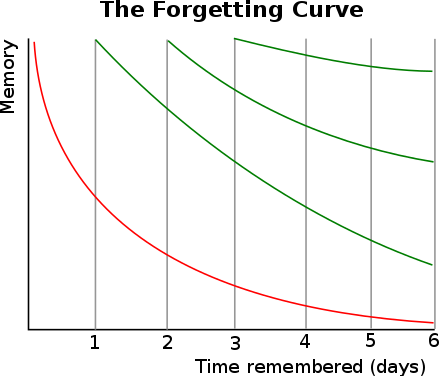
\includegraphics[width=0.4\textwidth]{images/vergessenskurve.png}
    \caption{ebbinghaussche Vergessenskurve \protect}
    \label{fig:curve}
\end{figure}

Auffällig an dem Modell ist die exponentiell ähnliche Abnahmen des erlangten Wissens. Die rote Kurve beschreibt den Anteil an gemerktem Wissen ohne eine weitere Wiederholung. Ebbinghaus hält fest, dass er nach 20 Minuten nur noch in der Lage war, 60\% richtig wiederzugeben. Nach einer Stunde waren es noch 45\%. Einen Tag und sechs Tage danach lag das gemerkte Wissen nur noch bei 34\% bzw. 23\%. Über einen langen Zeitraum festigen sich nur rund 15\% des geübten Wissens. Wird der Lernprozess durch Wiederholungen (grüne Graphen) ergänzt, festigt sich das Thema mit der Zeit. Die Kurve flacht schneller ab und ist generell weniger steil \cite{Wiki:Vergessenskurve}.

Kritisiert wird das Modell von Forschern in Hinsicht auf das Selbstexperiment \cite{Wiki:Vergessenskurve}. Es wird hinterfragt, wie geeignet ein Selbstexperiment zur Erfassung des Erinnerungsvermögens ist und inwiefern äußere Ereignisse Einfluss auf das Ergebnis hatten. Das Ebbinghaus sinnlose Silbenreihen genutzt hat, wird ebenfalls kritisiert, da Neurologie und Gehirnforschung gezeigt haben, dass persönlich bedeutsame Themen anderen Vergessenskurven unterliegen \cite{Wiki:Vergessenskurve}. Damit wurde bewiesen, dass Vergessen abhängig vom zu verinnerlichen Wissen ist, was in den Selbstversuchen nicht berücksichtigt wurde. C. Michel und F. Novak haben in neuen Studien \cite{Wiki:Vergessenskurve} diese Komponente berücksichtigt und den Anteil an vergessenem Wissen nach 5 Tagen und 30 Tagen festgehalten. Am wenigsten wurden Prinzipien und Gesetzmäßigkeiten vergessen (1\% bzw. 5\% wurden vergessen). Gedichte konnten zu 75\% bzw. 50\% nach verstrichener Zeit wiedergegeben werden. 53\% bzw. 60\% von den zuvor erlernten Prosa wurden vergessen. Die von Ebbinghaus genutzten sinnlosen Silbenreihen werden am schnellsten Vergessen. Nach der Zeit konnten lediglich 22\% bzw. 20\% richtig wiedergegeben werden \cite{Wiki:Vergessenskurve}

Für die Applikation ist das Modell von Ebbinghaus trotz der Kritik eine gute Orientierung, weil Schüler ein Spektrum an unterschiedlichen Dingen lernen müssen. Es lohnt sich nicht, für alle Möglichkeiten unterschiedliche Vergessenskurven als Grundlage zu nehmen. Außerdem sind die Fälle für ein Programm schwer zu unterscheiden, weshalb von dem schlechtesten Fall ausgegangen werden sollte.

\subsection{Konzept von Spaced Repetition}
Nach der Entdeckung der ebbinghausschen Vergessenskurve folgten Ansätze für ein darauf basierendes Lernverfahren. Mit \textit{Spaced Repetition} sollte gegen das schnell abfallende Wissen gewirkt werden, indem die eingängliche Wiederholung mit weiteren unterstützt wird. Dabei wird der Abstand der nachfolgenden Wiederholungen regelmäßig erhöht, um sich an die sinkende Verfallsrate von gefestigten Wissen anzupassen. 

Die anfängliche Idee war es, Karteikarten in Boxen zu kategorisieren. Die Boxen wurden von eins bis fünf mit Zahlen, welchen den Fortschritt widerspiegeln, durchnummeriert. In der ersten Box sind die Karten, welche der Schüler am schlechtesten beherrscht. Wenn die Karteikarte erfolgreich wiedergegeben wurde, dann wird die Karte in die nächst höhere Box gelegt. Eine Karte aus der Box eins würde dann in die Box 2 gelegt werden. Wenn eine Karte nicht wiedergegeben werden kann, dann wird diese egal wo sie vorher war, wieder in die Box eins gelegt. Beim lernen werden die Karten in der ersten Box priorisiert, um auf die Schwächen zu fokussieren.

\textit{Cramming}, eine zur \textit{Spaced Repetition} adverse Lernmethode, in welcher über einen kurzen Zeitraum Wissen angeeignet wird, ist bei vielen Schülern die standard Lerntechnik. Die damit verbundenen negativen Aspekte sind von der Hand zu weisen. Da bei dieser Methode nötige Wiederholungen fehlen, steht angeeignetes Wissen nur temporär zur Verfügung, was mit den Erkenntnissen der ebbinghausschen Vergessenskurve übereinstimmt. Das ist besonders kritisch, wenn andere Themen darauf aufbauen. Wegen dieser Gründe, sollte von \textit{Cramming} abgesehen werden und auf \textit{Spaced Repetition} zurückgegriffen werden.

\subsection{Ergebnisse von Studien}
Es liegen diverse Studien vor, welche die Effektivität von \textit{Spaced Repetiton} analysieren und bestätigen \cite{PNAS:Synaptic}\cite{RD:SpacedRepetition}. Dabei fächern sich die Beweismethoden auf verschiedene Bereiche, darunter Gehirnscans, womit die Stärke von synaptischen Verbindungen analysiert wird und experimentelle Studien, in welchen mit Probanden diverse Lernmethoden verglichen werden.

A. Voice und A. Stirton haben in \cite{RD:SpacedRepetition} eine Software für die Probanden entwickelt, die auf dem \textit{Spaced Repetition} Prinzip aufbaut, und die Auswirkungen auf das Prüfungsergebnis analysiert. Dafür wurde je einer Gruppe von Thermodynamik-Studenten die Software direkt nach Start, nach einem Sechstel und nach einem Drittel des Jahres vorgestellt. Dazu wurde mit irregulären Erinnerungen über das Jahr verteilt auf die Anwendung aufmerksam gemacht. Neben der Applikation konnten die Schüler lernen, wie sie wollten. Am Ende des Lehrjahres folgte eine Prüfung des Lernstands. Anschließend wurden die Testergebnisse verglichen. Während in dem ersten Jahr kein signifikant besseres Ergebnis der App-Nutzer gegenüber den nicht App-Nutzer erkennbar ist, kristallisiert sich in den Ergebnissen der darauf folgenden Jahrgänge eine signifikante Verbesserung der Lernleistung heraus. Ergänzend zur Prüfung folgte nach den Ferien ein unangekündigter Test, mit welchen das Langzeitpotenzial getestet wurde. Generell lagen schlechtere Ergebnisse der Schüler nach den Ferien vor, was mit dem Prinzip der ebbinghausschen Vergessenskurve übereinstimmt. Im Vergleich zwischen Nutzern und Nichtnutzern zeigten die Nutzer ein signifikant höheres Ergebnis, was das Langzeitpotenzial von \textit{Spaced Repetition} bestätigt.

In \cite{PNAS:Synaptic} untersuchen E. A. Kramár et al. die Stärke der Synapsenverbindungen in Hinblick auf das Langzeitpotenzial. Dafür wurden Synapsen eines Rattenhippocampus angeregt. Nach regelmäßigen Abständen wird die ursprüngliche Verbindung neu stimuliert. Dabei ging eine Steigerung Potenzierung nach 60 und 90 Minuten hervor. Eine erneute Stimulierung nach 10 oder 20 Minuten hat eine vergleichsweise minimale Steigerung. Des Weiteren hat die Studie festgestellt, dass eine dritte und vierte Stimulierung nach jeweiligen 60 Minuten kaum bis keine Auswirkungen auf die Langzeitpotenzierung hat, was einen steigenden Wiederholungsintervall impliziert. Ein Anstieg an Synapsen konnte von den Forschern ebenfalls nachgewiesen werden.

\section{Dart und Flutter}
\label{dart_flutter}
Dart ist eine von Google entwickelte Programmiersprache, welche auf Anwendungsentwicklung fokussiert ist, aber auch für Server genutzt werden kann. Anwendungen, die mit Dart programmiert werden, können Mobile Applikationen, Webseiten oder Desktop-Anwendungen sein. Dart implementiert viele herkömmliche Programmierpraktiken, wie Objektorientierung, Klassen und automatisierter Garbage Collection. Dart erschien erstmals am 10 Oktober 2011.

Das Beispiel \ref{lst:beispiel} zeigt rudimentäre Elemente von Dart. Es lassen sich viele Gleichheiten mit Programmiersprachen wie C\# und Java erkennen. Der Einstiegspunkt in das Programm ist in Dart ein wenig leichter gestaltet. Auffällig ist die für Dart typische dynamische Variablen Deklaration mit \texttt{final} für Variablen, welche einen konstanten Wert beibehalten. Ebenfalls zeigt die Zeile, dass bei Klasseninitialiserungen \textit{named parameter} angegeben werden. Jedoch ist dies nur der Fall, wenn in den Parameterklammern des Konstruktors geschweifte Klammern angegeben werden. Damit werden die Paramter zu optionalen namentlichen Parametern und müssen nicht angegeben werden. Das Schlüsselwort \texttt{required} wirkt gegensätzlich, sodass der Parameter doch angegeben werden muss. In Kombination aus geschweiften Klammern und dem Aufruf von Attributen, wird eine verkürzte Schreibweise für anfängliche Wertzuweisungen ermöglicht. In dem Beispiel \ref{lst:beispiel} wird das Attribut in den Konstrukt der Klasse \texttt{Zaehler} direkt mit dem Wert 100 initialisiert.

Die dynamische Syntax spiegelt sich auch in Dart-Methoden wieder. Rückgabewerte sind optional und es muss kein Schlüsselwort für Methoden angegeben werden, wie es in Python der Fall ist. Der Name und die Parameterklammern reichen aus. Die Rückgabe eines Wertes lässt sich auf zwei Weisen erreichen. Die herkömmliche Version lässt sich auch in C\# und Java finden. Dafür wird in dem Methodenkörper mit \texttt{return} ein Wert wiedergeben. Dafür hat Dart ebenfalls eine verkürzte Schreibweise. Mit \texttt{=>} wird der Ausdruck \texttt{{ return expr; }} abgekürzt. Damit sind geschweifte Klammern nicht mehr von Nöten und der Wert, welche aus der Zeile hervorgeht, wird von der Methode ausgegeben. Hierbei ist zu beachten, dass die verkürzte Schreibweise nur dann benutzt werden darf, wenn nur eine Zeile folgt. Für mehrere Zeilen muss auf die gewohnte Schreibweise zurückgegriffen werden. Dafür ist es genauso möglich nichts zurückzugeben, somit kann \texttt{=>} auch für \texttt{void}-Methoden genutzt werden.

\begin{lstlisting}[caption={Dart Beispiel},captionpos=b,label={lst:beispiel},numbers=left,frame=none,escapechar=|]
void main() {
  final b = Zaehler(amount: 100);
  b.alleFuenfAusgeben();
}

class Zaehler {
  int amount;

  Zaehler({required this.amount});

  alleFuenfAusgeben() {
    for (int i = 0; i < amount; i++) {
      if (fuenffach(i)) {
        print('hello ${i + 1}');
      }
    }
  }

  fuenffach(int zahl) => (zahl + 1) % 5 == 0;
}
\end{lstlisting}

Am 4 Dezember, 2018 wurde das \textit{open-source software development kit} Flutter in seiner ersten stabilen Version von Google veröffentlicht. Flutter umfasst ein komplettes \textit{Framwork} mit vorgefertigten \textit{Widgets} und \textit{Tools}. Eine mit Flutter programmierte Anwendung besteht aus vielen Widgets, welche auch wieder \textit{Widgets} beinhalten können. \textit{Buttons} oder \textit{Textfields} beispielsweise auch \textit{Widgets}. Kompiliert wird die Anwendung zu nativen \textit{Code}, entweder durch \textit{ahead-of-time} oder \textit{just-in-time} Kompilation. Bis zu Flutter 2 waren Programme für Android und IOS verfügbar. Mit der neuen Version vom 3 März 2021 wurden die Zielplattformen um Web, Windows, Linux und macOS ergänzt.

Trotz, dass Flutter relativ neu ist, haben Unternehmen unterschiedlichster Branchen Flutter adaptiert \cite{Flutter:Usage}. Da es ein Produkt aus dem Hause Google ist, wird es dort auch für Applikationen wie \textit{Google Pay} genutzt. Ein weiterer Vertreter des amerikanischen Markts ist Ebay, welcher für ebay motors eine Ebay ähnliche Applikation für Auto bezogene Themen mit Flutter entwickelt hat. Das Anwendungsentwicklungsteam des deutschen Autoherstellers BMW vertraut auf Flutter für die Autos begleitende Applikation. Flutter wird auch von asiatischen Unternehmen genutzt. Die Tech-Unternehmen Alibaba, Tencent, ByteDance und Toyota bedienen sich ebenfalls an dem Flutter Framework. Die Entwickler der aufgelisteten Unternehmen sprechen laut \cite{Flutter:Usage} von Leistungs- und Effektivitätssteigerungen. 
